\section{hdass\-Album Class Reference}
\label{classhdassAlbum}\index{hdassAlbum@{hdassAlbum}}
{\tt \#include $<$hdassalbum.h$>$}

Inheritance diagram for hdass\-Album:\begin{figure}[H]
\begin{center}
\leavevmode
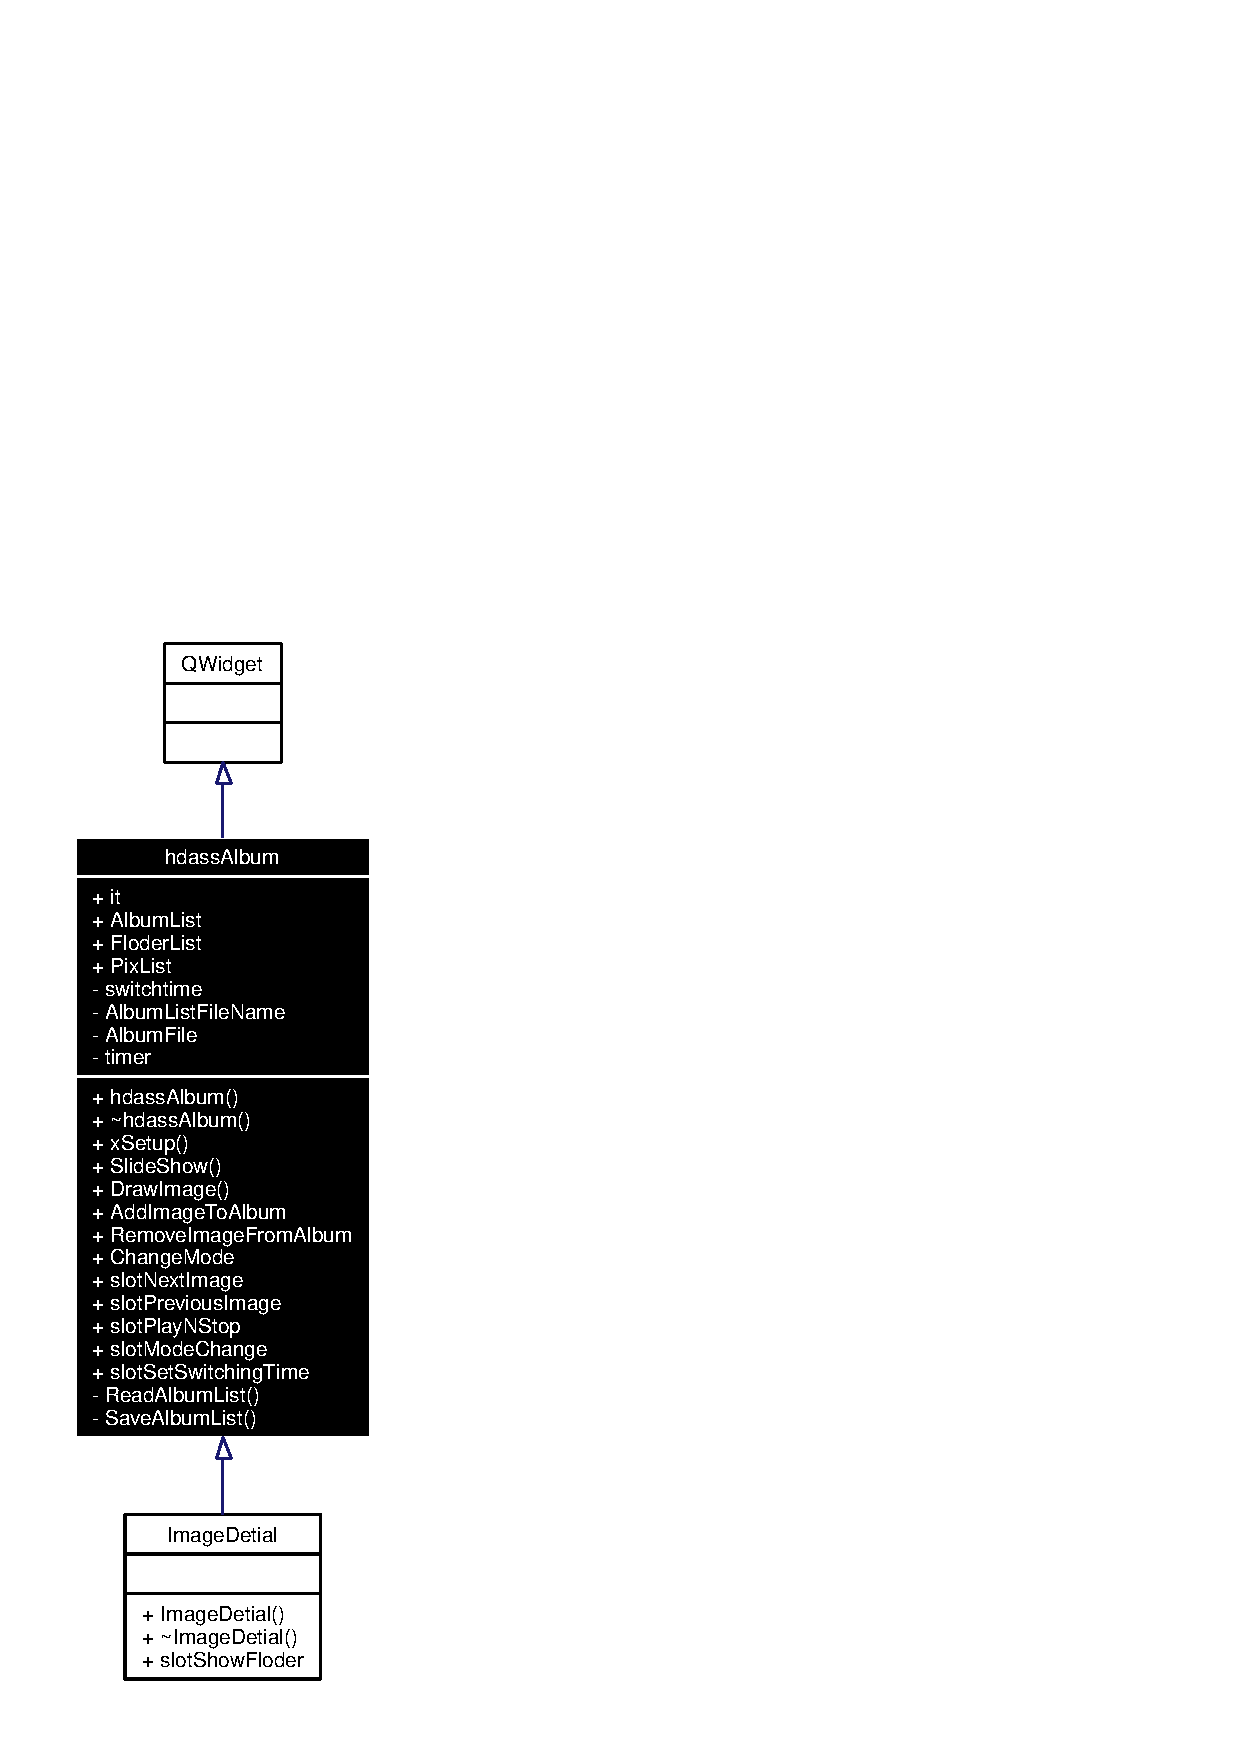
\includegraphics[width=89pt]{classhdassAlbum__inherit__graph}
\end{center}
\end{figure}
Collaboration diagram for hdass\-Album:\begin{figure}[H]
\begin{center}
\leavevmode
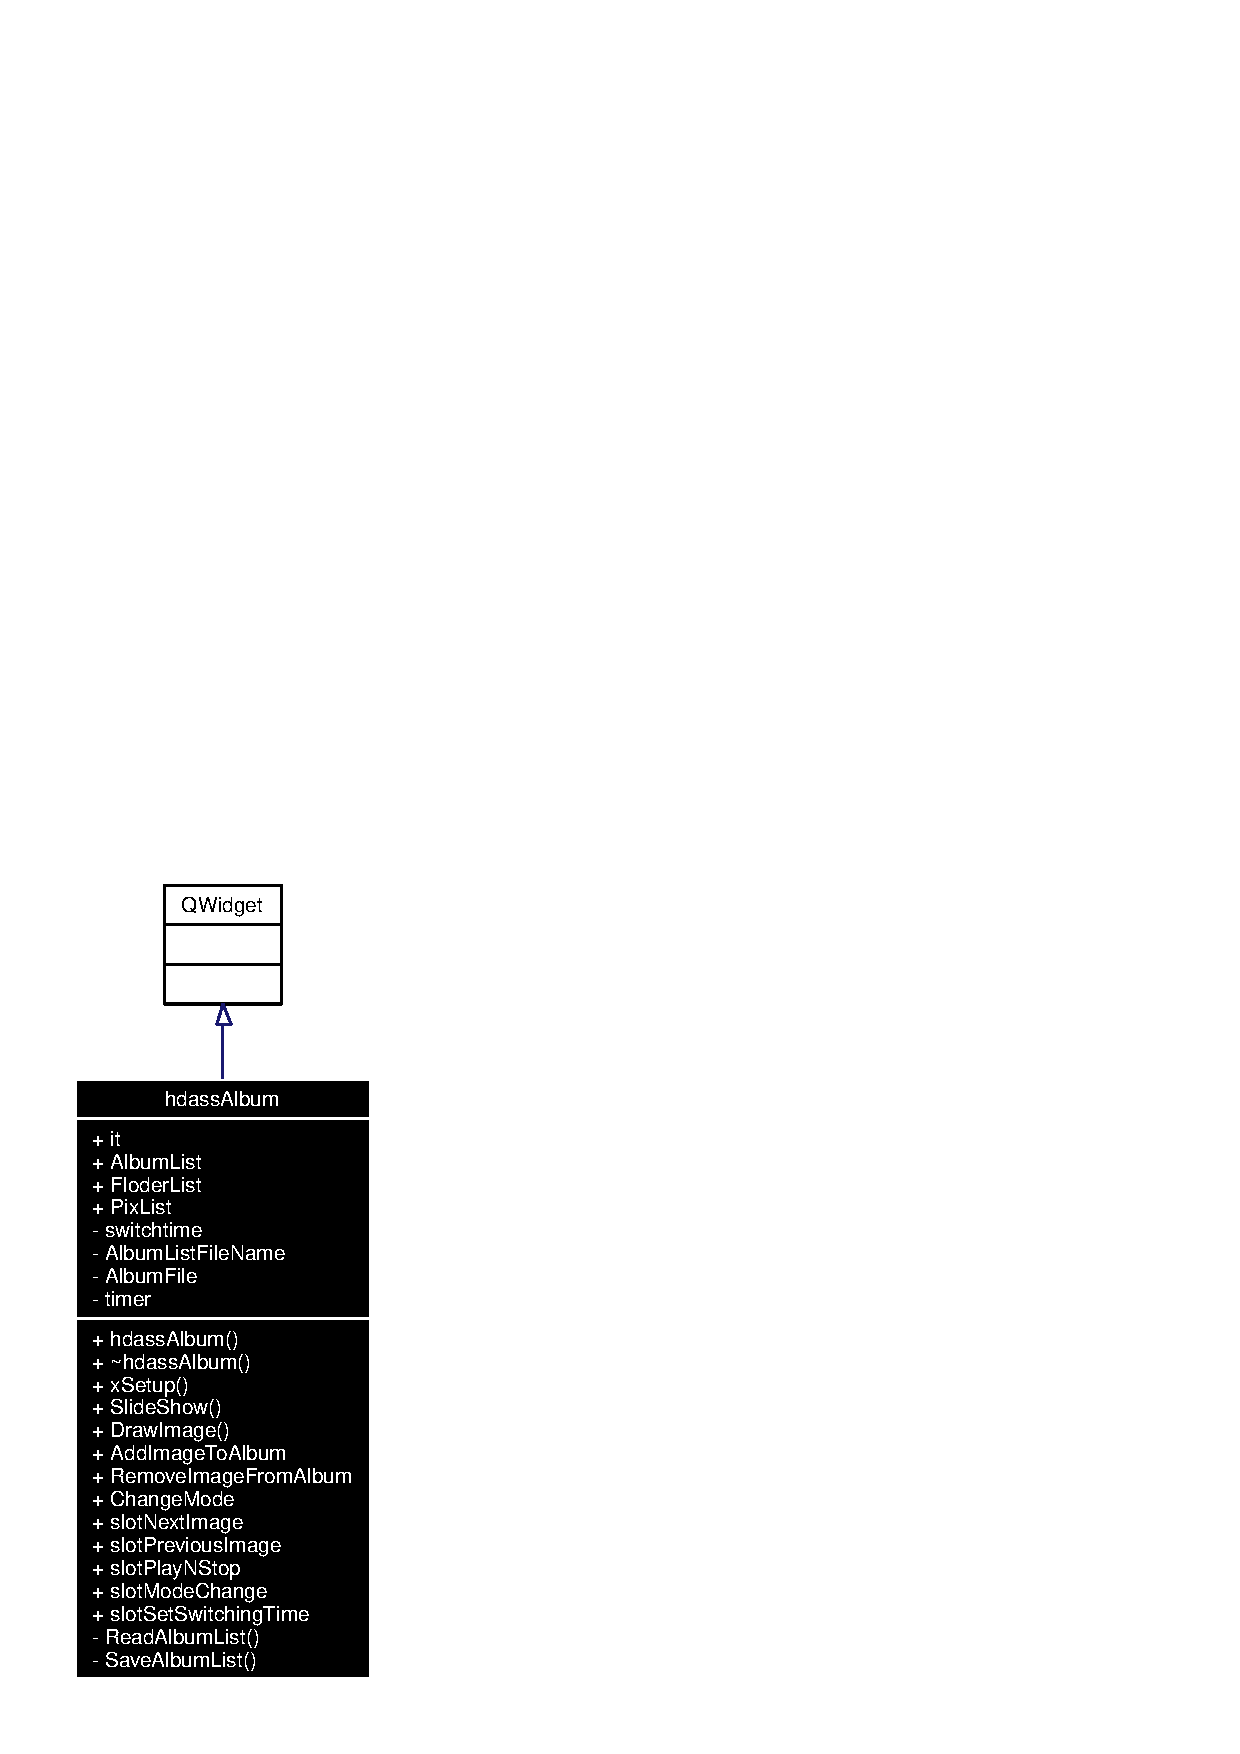
\includegraphics[width=89pt]{classhdassAlbum__coll__graph}
\end{center}
\end{figure}


\subsection{Detailed Description}
\begin{Desc}
\item[Author:]root \end{Desc}




Definition at line 34 of file hdassalbum.h.\subsection*{Public Slots}
\begin{CompactItemize}
\item 
void {\bf Add\-Image\-To\-Album} (KURL addimage)
\item 
void {\bf Remove\-Image\-From\-Album} (KURL removeimage)
\item 
void {\bf Change\-Mode} ({\bf Album\-Mode} mode)
\item 
void {\bf slot\-Next\-Image} ()
\item 
void {\bf slot\-Previous\-Image} ()
\item 
void {\bf slot\-Play\-NStop} ()
\item 
void {\bf slot\-Mode\-Change} (int)
\item 
void {\bf slot\-Set\-Switching\-Time} (int time)
\end{CompactItemize}
\subsection*{Public Member Functions}
\begin{CompactItemize}
\item 
{\bf hdass\-Album} ({\bf QWidget} $\ast$parent=0, const char $\ast$name=0)
\item 
{\bf $\sim$hdass\-Album} ()
\item 
void {\bf x\-Setup} ()
\item 
void {\bf Slide\-Show} ()
\item 
void {\bf Draw\-Image} (QPixmap pix)
\end{CompactItemize}
\subsection*{Public Attributes}
\begin{CompactItemize}
\item 
KURL::List::Const\-Iterator {\bf it}
\item 
KURL::List {\bf Album\-List}
\item 
KURL::List {\bf Floder\-List}
\item 
QPtr\-List$<$ QPixmap $>$ {\bf Pix\-List}
\end{CompactItemize}
\subsection*{Private Types}
\begin{CompactItemize}
\item 
enum {\bf Album\-Mode} \{ {\bf Album} = 0, 
{\bf Clock}
 \}
\end{CompactItemize}
\subsection*{Private Member Functions}
\begin{CompactItemize}
\item 
void {\bf Read\-Album\-List} (QString filename)
\item 
void {\bf Save\-Album\-List} ()
\end{CompactItemize}
\subsection*{Private Attributes}
\begin{CompactItemize}
\item 
int {\bf switchtime}
\item 
QString {\bf Album\-List\-File\-Name}
\item 
QFile $\ast$ {\bf Album\-File}
\item 
QTimer $\ast$ {\bf timer}
\end{CompactItemize}


\subsection{Member Enumeration Documentation}
\index{hdassAlbum@{hdass\-Album}!AlbumMode@{AlbumMode}}
\index{AlbumMode@{AlbumMode}!hdassAlbum@{hdass\-Album}}
\subsubsection{\setlength{\rightskip}{0pt plus 5cm}enum {\bf hdass\-Album::Album\-Mode}\hspace{0.3cm}{\tt  [private]}}\label{classhdassAlbum_hdassAlbumy2}


\begin{Desc}
\item[Enumeration values: ]\par
\begin{description}
\index{Album@{Album}!hdassAlbum@{hdassAlbum}}\index{hdassAlbum@{hdassAlbum}!Album@{Album}}\item[{\em 
Album\label{classhdassAlbum_hdassAlbumy2hdassAlbumy0}
}]\index{Clock@{Clock}!hdassAlbum@{hdassAlbum}}\index{hdassAlbum@{hdassAlbum}!Clock@{Clock}}\item[{\em 
Clock\label{classhdassAlbum_hdassAlbumy2hdassAlbumy1}
}]\end{description}
\end{Desc}



Definition at line 37 of file hdassalbum.h.



\footnotesize\begin{verbatim}38 {
39   Album=0,
40   Clock     
41 };
\end{verbatim}\normalsize 


\subsection{Constructor \& Destructor Documentation}
\index{hdassAlbum@{hdass\-Album}!hdassAlbum@{hdassAlbum}}
\index{hdassAlbum@{hdassAlbum}!hdassAlbum@{hdass\-Album}}
\subsubsection{\setlength{\rightskip}{0pt plus 5cm}hdass\-Album::hdass\-Album ({\bf QWidget} $\ast$ {\em parent} = 0, const char $\ast$ {\em name} = 0)}\label{classhdassAlbum_hdassAlbuma0}




Definition at line 26 of file hdassalbum.cpp.

References x\-Setup().



\footnotesize\begin{verbatim}27  : QWidget(parent, name)
28 {
29    xSetup();
30 }
\end{verbatim}\normalsize 


Here is the call graph for this function:\begin{figure}[H]
\begin{center}
\leavevmode
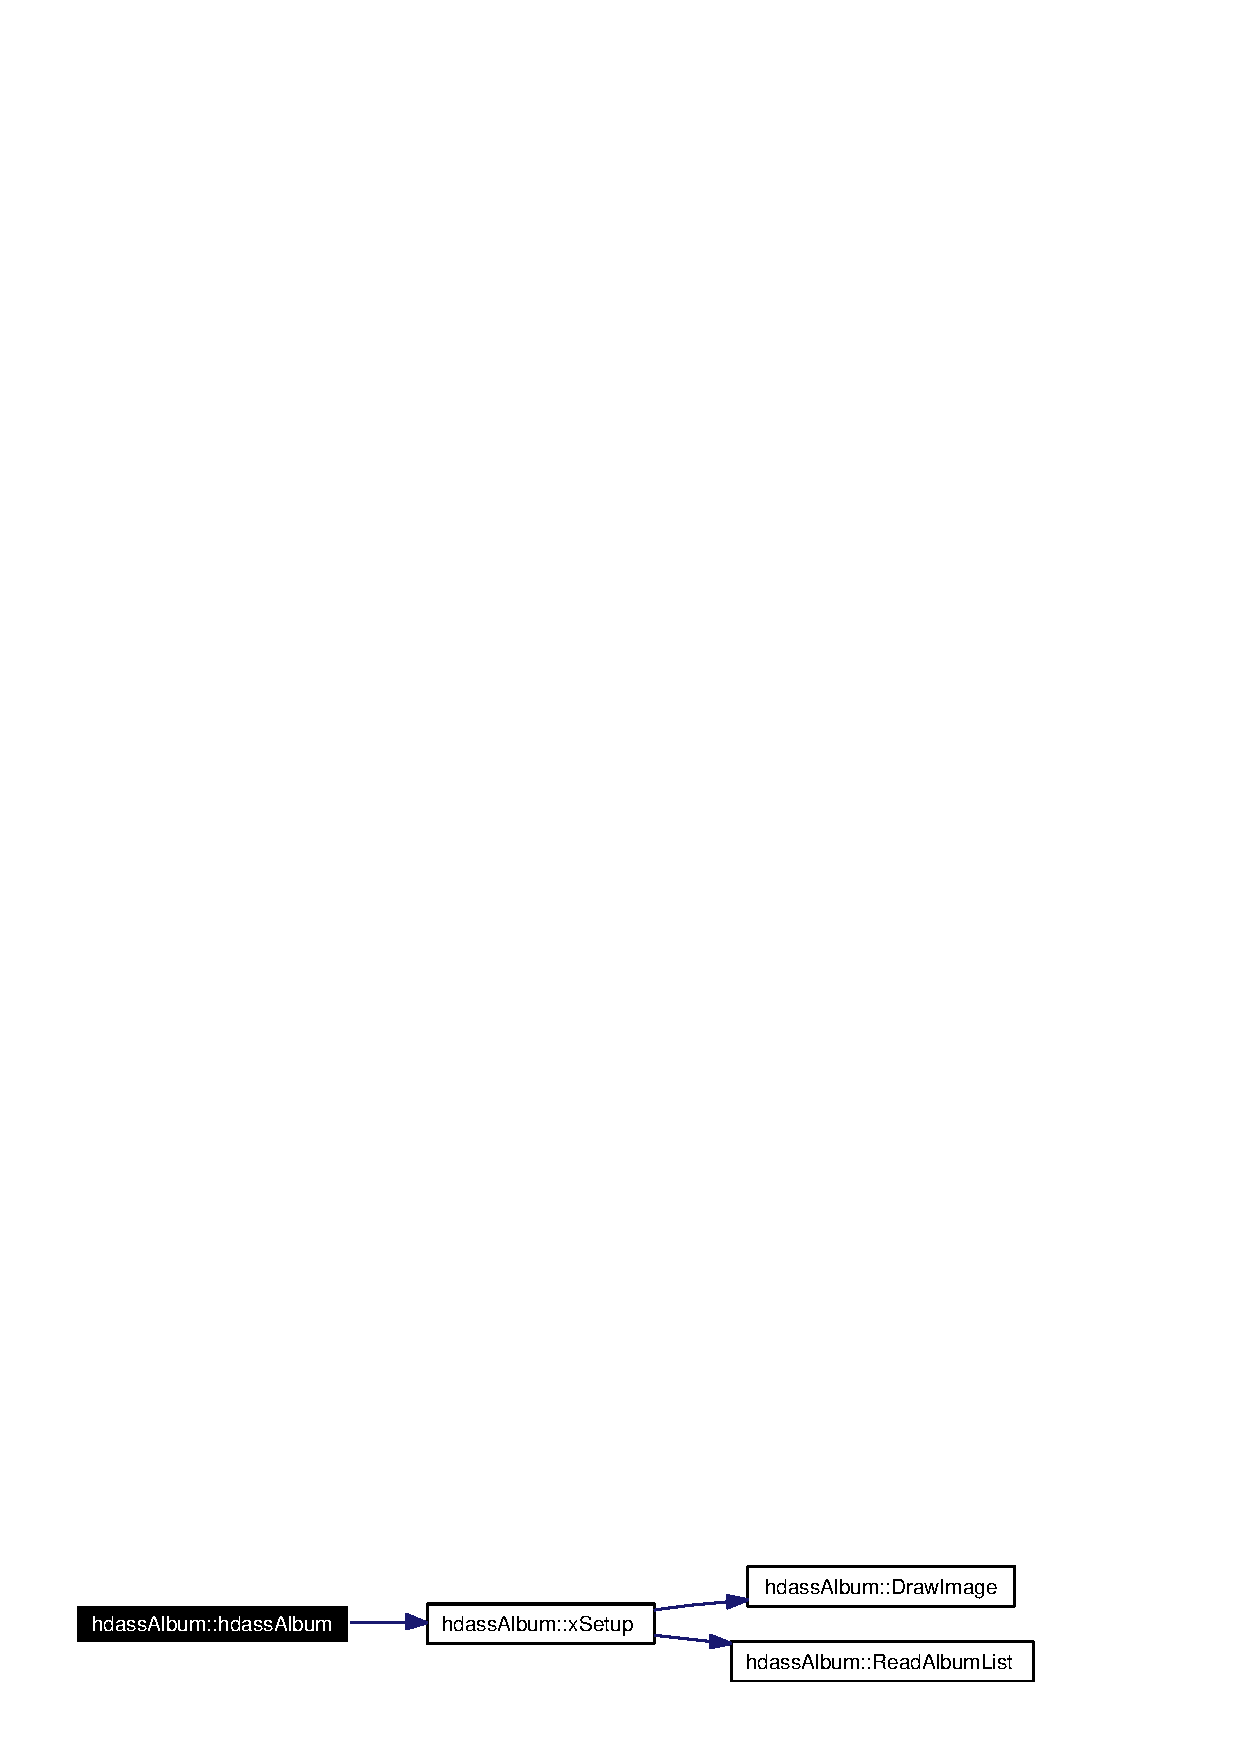
\includegraphics[width=248pt]{classhdassAlbum_hdassAlbuma0_cgraph}
\end{center}
\end{figure}
\index{hdassAlbum@{hdass\-Album}!~hdassAlbum@{$\sim$hdassAlbum}}
\index{~hdassAlbum@{$\sim$hdassAlbum}!hdassAlbum@{hdass\-Album}}
\subsubsection{\setlength{\rightskip}{0pt plus 5cm}hdass\-Album::$\sim${\bf hdass\-Album} ()}\label{classhdassAlbum_hdassAlbuma1}




Definition at line 33 of file hdassalbum.cpp.



\footnotesize\begin{verbatim}34 {
35 
36 }
\end{verbatim}\normalsize 


\subsection{Member Function Documentation}
\index{hdassAlbum@{hdass\-Album}!AddImageToAlbum@{AddImageToAlbum}}
\index{AddImageToAlbum@{AddImageToAlbum}!hdassAlbum@{hdass\-Album}}
\subsubsection{\setlength{\rightskip}{0pt plus 5cm}void hdass\-Album::Add\-Image\-To\-Album (KURL {\em addimage})\hspace{0.3cm}{\tt  [slot]}}\label{classhdassAlbum_ImageDetiali1}




Definition at line 60 of file hdassalbum.cpp.

References Album\-List.



\footnotesize\begin{verbatim}61 {
62    AlbumList<<addimage;
63 }
\end{verbatim}\normalsize 
\index{hdassAlbum@{hdass\-Album}!ChangeMode@{ChangeMode}}
\index{ChangeMode@{ChangeMode}!hdassAlbum@{hdass\-Album}}
\subsubsection{\setlength{\rightskip}{0pt plus 5cm}void hdass\-Album::Change\-Mode ({\bf Album\-Mode} {\em mode})\hspace{0.3cm}{\tt  [slot]}}\label{classhdassAlbum_ImageDetiali3}




Definition at line 69 of file hdassalbum.cpp.



\footnotesize\begin{verbatim}70 {
71 
72 }
\end{verbatim}\normalsize 
\index{hdassAlbum@{hdass\-Album}!DrawImage@{DrawImage}}
\index{DrawImage@{DrawImage}!hdassAlbum@{hdass\-Album}}
\subsubsection{\setlength{\rightskip}{0pt plus 5cm}void hdass\-Album::Draw\-Image (QPixmap {\em pix})}\label{classhdassAlbum_ImageDetiala4}




Definition at line 154 of file hdassalbum.cpp.

Referenced by slot\-Next\-Image(), slot\-Previous\-Image(), Image\-Detial::slot\-Show\-Floder(), and x\-Setup().



\footnotesize\begin{verbatim}155 {
156    
157    
158    int width ,height;
159    width=pix.width();
160    height=pix.height();
161    
162    QPixmap draw(QSize(800,540));
163    QPainter p(&draw);
164 
165    p.fillRect(0,0,800,540,Qt::black);
166    if(width<800&&height<540)
167    {
168        //DAVID draw image at center
169        p.drawPixmap((400-width/2),(270-height/2),pix);
170    }
171 
172    else
173    {
174         if(11*width>20*height)
175         {
176                 int newheight=(800*height/width);
177                 QImage rescale=pix.convertToImage().scale(800,newheight);
178                 p.drawImage(0,270-newheight/2,rescale);
179                 
180         } 
181         else
182         {
183                 int newwidth=(540*width/height);
184                 QImage rescale=pix.convertToImage().scale(newwidth,540);
185                 p.drawImage((400-newwidth/2),0,rescale);
186         }
187    }    
188    p.end();
189    setBackgroundPixmap(draw);
190 }
\end{verbatim}\normalsize 
\index{hdassAlbum@{hdass\-Album}!ReadAlbumList@{ReadAlbumList}}
\index{ReadAlbumList@{ReadAlbumList}!hdassAlbum@{hdass\-Album}}
\subsubsection{\setlength{\rightskip}{0pt plus 5cm}void hdass\-Album::Read\-Album\-List (QString {\em filename})\hspace{0.3cm}{\tt  [private]}}\label{classhdassAlbum_hdassAlbumd0}




Definition at line 77 of file hdassalbum.cpp.

References Album\-File, Album\-List, and it.

Referenced by x\-Setup().



\footnotesize\begin{verbatim}78 {
79         //DAVID open the file
80         AlbumFile=new QFile(filepath);
81         if(AlbumFile->open(IO_ReadOnly))
82         {
83                 //Read KURL from file to KURLList
84                 QTextStream stream( AlbumFile );
85                 while(!stream.atEnd())
86                 {
87                         KURL url(stream.readLine());
88                         //kdDebug()<<url.path();
89                         AlbumList<<url;
90                 }
91         }
92         else
93         {
94                 kdDebug()<<"hdassAlbum::ReadAlbumList ::: file not opened!!";
95         }
96         it=AlbumList.begin();
97 }
\end{verbatim}\normalsize 
\index{hdassAlbum@{hdass\-Album}!RemoveImageFromAlbum@{RemoveImageFromAlbum}}
\index{RemoveImageFromAlbum@{RemoveImageFromAlbum}!hdassAlbum@{hdass\-Album}}
\subsubsection{\setlength{\rightskip}{0pt plus 5cm}void hdass\-Album::Remove\-Image\-From\-Album (KURL {\em removeimage})\hspace{0.3cm}{\tt  [slot]}}\label{classhdassAlbum_ImageDetiali2}




Definition at line 65 of file hdassalbum.cpp.

References Album\-List.



\footnotesize\begin{verbatim}66 {
67   AlbumList.remove(removeimage);
68 }
\end{verbatim}\normalsize 
\index{hdassAlbum@{hdass\-Album}!SaveAlbumList@{SaveAlbumList}}
\index{SaveAlbumList@{SaveAlbumList}!hdassAlbum@{hdass\-Album}}
\subsubsection{\setlength{\rightskip}{0pt plus 5cm}void hdass\-Album::Save\-Album\-List ()\hspace{0.3cm}{\tt  [private]}}\label{classhdassAlbum_hdassAlbumd1}




Definition at line 99 of file hdassalbum.cpp.



\footnotesize\begin{verbatim}100 {
101 
102 }
\end{verbatim}\normalsize 
\index{hdassAlbum@{hdass\-Album}!SlideShow@{SlideShow}}
\index{SlideShow@{SlideShow}!hdassAlbum@{hdass\-Album}}
\subsubsection{\setlength{\rightskip}{0pt plus 5cm}void hdass\-Album::Slide\-Show ()}\label{classhdassAlbum_ImageDetiala3}




Definition at line 148 of file hdassalbum.cpp.

References switchtime, and timer.



\footnotesize\begin{verbatim}149 {
150      qWarning("hdassAlbum::SlideShow()!!");
151      timer->start(switchtime*1000,FALSE);
152 }
\end{verbatim}\normalsize 
\index{hdassAlbum@{hdass\-Album}!slotModeChange@{slotModeChange}}
\index{slotModeChange@{slotModeChange}!hdassAlbum@{hdass\-Album}}
\subsubsection{\setlength{\rightskip}{0pt plus 5cm}void hdass\-Album::slot\-Mode\-Change (int)\hspace{0.3cm}{\tt  [slot]}}\label{classhdassAlbum_ImageDetiali7}




Definition at line 73 of file hdassalbum.cpp.



\footnotesize\begin{verbatim}74 {
75 
76 }
\end{verbatim}\normalsize 
\index{hdassAlbum@{hdass\-Album}!slotNextImage@{slotNextImage}}
\index{slotNextImage@{slotNextImage}!hdassAlbum@{hdass\-Album}}
\subsubsection{\setlength{\rightskip}{0pt plus 5cm}void hdass\-Album::slot\-Next\-Image ()\hspace{0.3cm}{\tt  [slot]}}\label{classhdassAlbum_ImageDetiali4}




Definition at line 117 of file hdassalbum.cpp.

References Album\-List, Draw\-Image(), and it.

Referenced by x\-Setup().



\footnotesize\begin{verbatim}118 {
119         //DAVID Read Image
120         it++;
121         if(it!=AlbumList.end())
122         {
123                 KURL url((*it).url());
124                 QPixmap pix;
125                 pix.load(url.path());
126                 DrawImage(pix);
127         }
128 }
\end{verbatim}\normalsize 
\index{hdassAlbum@{hdass\-Album}!slotPlayNStop@{slotPlayNStop}}
\index{slotPlayNStop@{slotPlayNStop}!hdassAlbum@{hdass\-Album}}
\subsubsection{\setlength{\rightskip}{0pt plus 5cm}void hdass\-Album::slot\-Play\-NStop ()\hspace{0.3cm}{\tt  [slot]}}\label{classhdassAlbum_ImageDetiali6}




Definition at line 130 of file hdassalbum.cpp.

References switchtime, and timer.



\footnotesize\begin{verbatim}131 {
132         if(timer->isActive ())
133         {
134                 timer->stop();
135         }
136         else
137         {
138                 timer->start(switchtime*1000,FALSE);
139         }
140 }
\end{verbatim}\normalsize 
\index{hdassAlbum@{hdass\-Album}!slotPreviousImage@{slotPreviousImage}}
\index{slotPreviousImage@{slotPreviousImage}!hdassAlbum@{hdass\-Album}}
\subsubsection{\setlength{\rightskip}{0pt plus 5cm}void hdass\-Album::slot\-Previous\-Image ()\hspace{0.3cm}{\tt  [slot]}}\label{classhdassAlbum_ImageDetiali5}




Definition at line 104 of file hdassalbum.cpp.

References Album\-List, Draw\-Image(), and it.



\footnotesize\begin{verbatim}105 {
106         //DAVID Read Image
107         it--;
108         if(it!=AlbumList.end())
109         {
110                 KURL url((*it).url());
111                 QPixmap pix;
112                 pix.load(url.path());
113                 DrawImage(pix);
114         }
115 }
\end{verbatim}\normalsize 
\index{hdassAlbum@{hdass\-Album}!slotSetSwitchingTime@{slotSetSwitchingTime}}
\index{slotSetSwitchingTime@{slotSetSwitchingTime}!hdassAlbum@{hdass\-Album}}
\subsubsection{\setlength{\rightskip}{0pt plus 5cm}void hdass\-Album::slot\-Set\-Switching\-Time (int {\em time})\hspace{0.3cm}{\tt  [slot]}}\label{classhdassAlbum_ImageDetiali8}




Definition at line 143 of file hdassalbum.cpp.

References switchtime.



\footnotesize\begin{verbatim}144 {
145   switchtime=time;
146 }
\end{verbatim}\normalsize 
\index{hdassAlbum@{hdass\-Album}!xSetup@{xSetup}}
\index{xSetup@{xSetup}!hdassAlbum@{hdass\-Album}}
\subsubsection{\setlength{\rightskip}{0pt plus 5cm}void hdass\-Album::x\-Setup ()}\label{classhdassAlbum_ImageDetiala2}




Definition at line 38 of file hdassalbum.cpp.

References Album\-List\-File\-Name, Draw\-Image(), Read\-Album\-List(), slot\-Next\-Image(), switchtime, and timer.

Referenced by hdass\-Album().



\footnotesize\begin{verbatim}39 {
40   //DAVID Read album file list 
41   AlbumListFileName="AlbumList.txt";
42   ReadAlbumList(AlbumListFileName);
43   
44  
45 
46   //DAVID Set the switching time
47   switchtime=3;
48   //DAVID Set the timer
49   timer =new QTimer(this);
50   connect(timer,SIGNAL(timeout()),this,SLOT(slotNextImage()));
51   
52   //DAVID Draw a pix first
53   KURL url((*it).url());
54   QPixmap pix;
55   pix.load(url.path());
56   DrawImage(pix);
57   timer->stop();
58   
59 }
\end{verbatim}\normalsize 


Here is the call graph for this function:\begin{figure}[H]
\begin{center}
\leavevmode
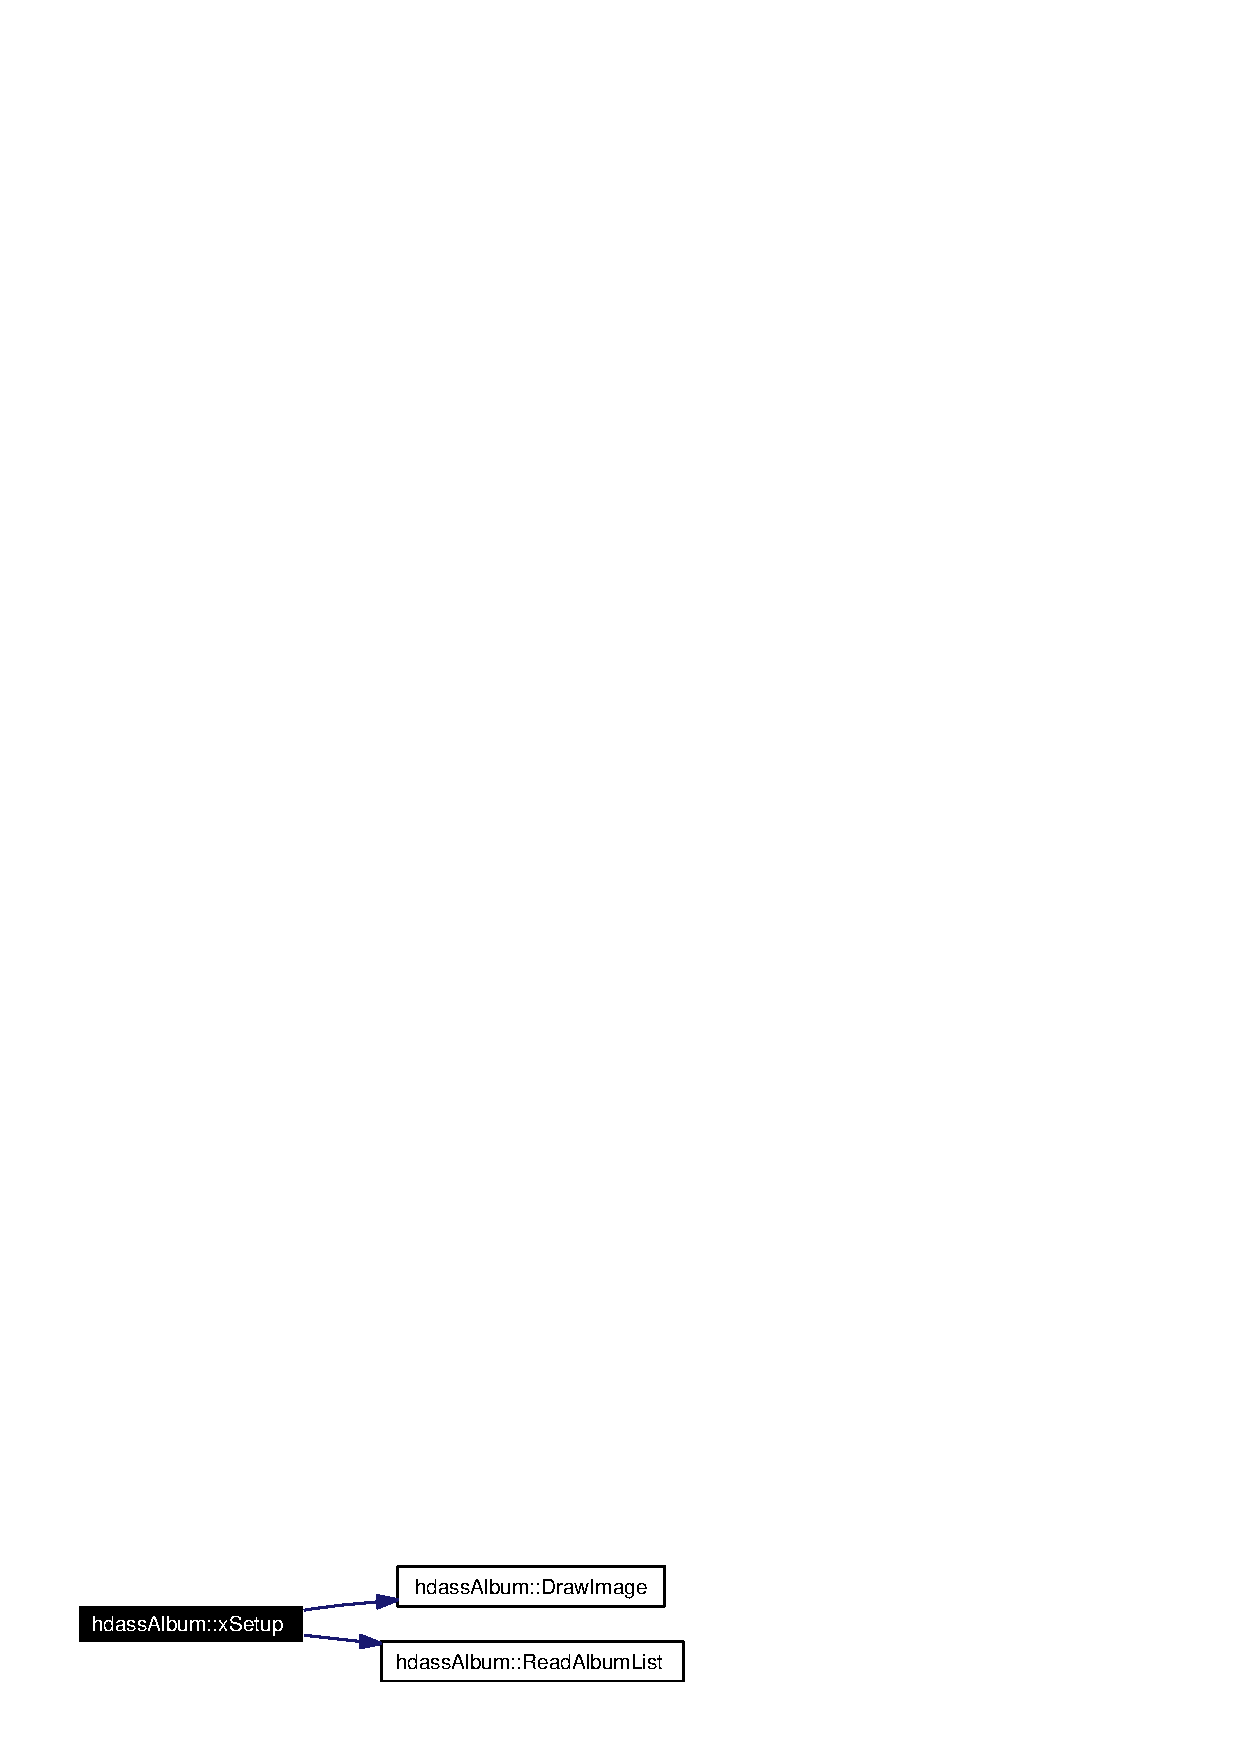
\includegraphics[width=164pt]{classhdassAlbum_ImageDetiala2_cgraph}
\end{center}
\end{figure}


\subsection{Member Data Documentation}
\index{hdassAlbum@{hdass\-Album}!AlbumFile@{AlbumFile}}
\index{AlbumFile@{AlbumFile}!hdassAlbum@{hdass\-Album}}
\subsubsection{\setlength{\rightskip}{0pt plus 5cm}QFile$\ast$ {\bf hdass\-Album::Album\-File}\hspace{0.3cm}{\tt  [private]}}\label{classhdassAlbum_hdassAlbumr2}




Definition at line 65 of file hdassalbum.h.

Referenced by Read\-Album\-List().\index{hdassAlbum@{hdass\-Album}!AlbumList@{AlbumList}}
\index{AlbumList@{AlbumList}!hdassAlbum@{hdass\-Album}}
\subsubsection{\setlength{\rightskip}{0pt plus 5cm}KURL::List {\bf hdass\-Album::Album\-List}}\label{classhdassAlbum_ImageDetialo1}




Definition at line 50 of file hdassalbum.h.

Referenced by Add\-Image\-To\-Album(), Read\-Album\-List(), Remove\-Image\-From\-Album(), slot\-Next\-Image(), and slot\-Previous\-Image().\index{hdassAlbum@{hdass\-Album}!AlbumListFileName@{AlbumListFileName}}
\index{AlbumListFileName@{AlbumListFileName}!hdassAlbum@{hdass\-Album}}
\subsubsection{\setlength{\rightskip}{0pt plus 5cm}QString {\bf hdass\-Album::Album\-List\-File\-Name}\hspace{0.3cm}{\tt  [private]}}\label{classhdassAlbum_hdassAlbumr1}




Definition at line 64 of file hdassalbum.h.

Referenced by x\-Setup().\index{hdassAlbum@{hdass\-Album}!FloderList@{FloderList}}
\index{FloderList@{FloderList}!hdassAlbum@{hdass\-Album}}
\subsubsection{\setlength{\rightskip}{0pt plus 5cm}KURL::List {\bf hdass\-Album::Floder\-List}}\label{classhdassAlbum_ImageDetialo2}




Definition at line 50 of file hdassalbum.h.\index{hdassAlbum@{hdass\-Album}!it@{it}}
\index{it@{it}!hdassAlbum@{hdass\-Album}}
\subsubsection{\setlength{\rightskip}{0pt plus 5cm}KURL::List::Const\-Iterator {\bf hdass\-Album::it}}\label{classhdassAlbum_ImageDetialo0}




Definition at line 49 of file hdassalbum.h.

Referenced by Read\-Album\-List(), slot\-Next\-Image(), and slot\-Previous\-Image().\index{hdassAlbum@{hdass\-Album}!PixList@{PixList}}
\index{PixList@{PixList}!hdassAlbum@{hdass\-Album}}
\subsubsection{\setlength{\rightskip}{0pt plus 5cm}QPtr\-List$<$QPixmap$>$ {\bf hdass\-Album::Pix\-List}}\label{classhdassAlbum_ImageDetialo3}




Definition at line 51 of file hdassalbum.h.\index{hdassAlbum@{hdass\-Album}!switchtime@{switchtime}}
\index{switchtime@{switchtime}!hdassAlbum@{hdass\-Album}}
\subsubsection{\setlength{\rightskip}{0pt plus 5cm}int {\bf hdass\-Album::switchtime}\hspace{0.3cm}{\tt  [private]}}\label{classhdassAlbum_hdassAlbumr0}




Definition at line 63 of file hdassalbum.h.

Referenced by Slide\-Show(), slot\-Play\-NStop(), slot\-Set\-Switching\-Time(), and x\-Setup().\index{hdassAlbum@{hdass\-Album}!timer@{timer}}
\index{timer@{timer}!hdassAlbum@{hdass\-Album}}
\subsubsection{\setlength{\rightskip}{0pt plus 5cm}QTimer$\ast$ {\bf hdass\-Album::timer}\hspace{0.3cm}{\tt  [private]}}\label{classhdassAlbum_hdassAlbumr3}




Definition at line 66 of file hdassalbum.h.

Referenced by Slide\-Show(), slot\-Play\-NStop(), and x\-Setup().

The documentation for this class was generated from the following files:\begin{CompactItemize}
\item 
{\bf hdassalbum.h}\item 
{\bf hdassalbum.cpp}\end{CompactItemize}
